\subsection{Overview}

The high level architecture is composed of three layers.The most external is the client layer, it provides the interfaces that allows user-system interactions: the web application, the mobile application and the car system. The second layer is composed by an application logic server that will handle the users requests and that will send the requested data to the first layer components, this layer will also send modification data requests to the third layer. The third layer is composed by a database and his DBMS, this layer will handle the user data, requests data and cars data.

\begin{figure}[hp]
\centering
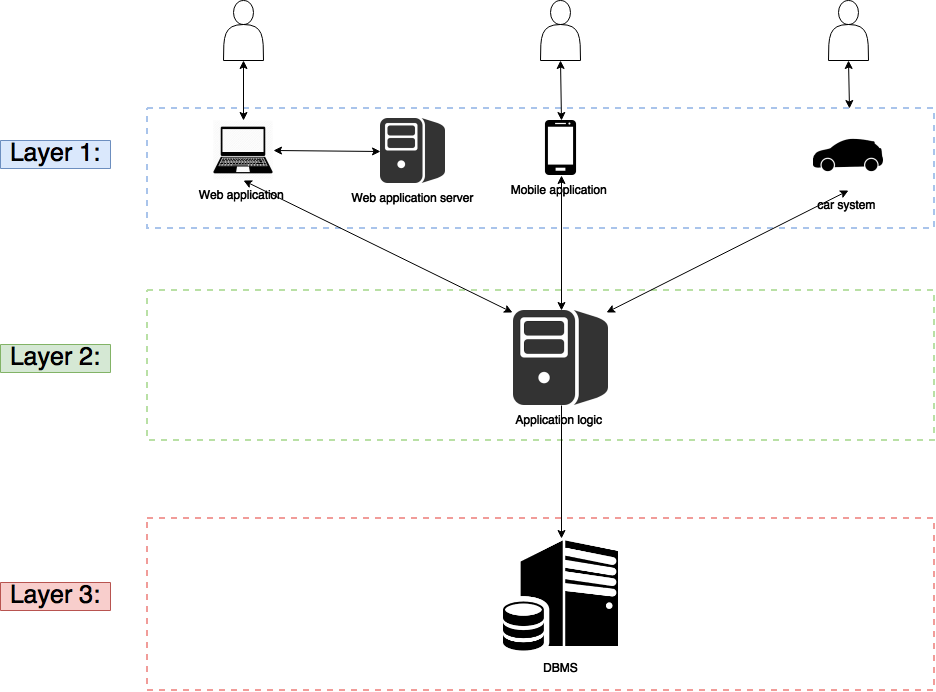
\includegraphics[width=470 pt]{resources/Architectural_structure.png}
\caption{\label{fig:layer}Layers architecture}
\end{figure}

\newpage

\subsection{High level components and their interaction}
In the first level we find two components, the client and the car system. The client is composed of a web application and a mobile application.The web application has to interact with a dedicated server in order to work properly, it should be implemented in java script and HTML and it should have its standalone logic, making to the server only the request for getting data about cars and the map, the request of starting a reservation and the requests of updating the account information. The mobile application should have his standalone logic as well and it will make to the server the same requests as the web application. The car system will be a java application accessible from the car display, through which the user can insert the pin, report damages and end the rent.The request will be send to the server. 
At the second level there is the server,which should be written in php and should have an event driven architecture because it should handle multiple requests at the same time asynchronously. The server interacts with the client by sending notifications about the payments and requesting periodically the position. The server interacts with the car requiring lock/unlock doors and enable engine.The server also requires information such as the position, the remaining charge, the number of passengers and if the car is plugged or not to a charging station.  
At the third level we find the DBMS server that handles a SQL database.
The server interacts with the DBMS with some fetch data request and with some data update requests.
\\

\begin{figure}[hp]
\centering
\includegraphics[width=420 pt]{resources/High_components.png}
\caption{\label{fig:high_component}High level component diagram.}
\end{figure}


\newpage
\subsection{Component view}
\begin{figure}[hp]
\centering
\includegraphics[width=490 pt]{resources/component.jpg}
\caption{\label{fig:component}Component diagram.}
\end{figure}

\newpage
\subsection{Deployment view}
\begin{figure}[hp]
\centering
\includegraphics[width=470 pt]{resources/deploy.jpg}
\caption{\label{fig:deploy}Deployment diagram.}
\end{figure}

\newpage
\subsection{Runtime view}

\subsubsection*{Reserve a car}
\begin{figure}[hp]
\centering
\includegraphics[width=455 pt]{resources/RunView.jpg}
\caption{\label{fig:reserve}Runtime diagrams for reserve a car.}
\end{figure}

\newpage
\subsubsection*{Rent a car}
\begin{figure}[hp]
\centering
\includegraphics[width=400 pt]{resources/RunView2.jpg}
\caption{\label{fig:startrent}Runtime diagrams for start a rent.}
\end{figure}

\newpage
\subsubsection*{End a rent}
\begin{figure}[hp]
\centering
\includegraphics[width=370 pt]{resources/RunView3.jpg}
\caption{\label{fig:endrent}Runtime diagrams for end a rent.}
\end{figure}


\newpage
\subsection{Component interfaces}
\begin{figure}[hp]
\centering
\includegraphics[width=455 pt]{resources/interface.jpg}
\caption{\label{fig:interface}Component interface diagram.}
\end{figure}


\newpage
\subsection{Selected architectural styles and patterns}
\subparagraph{Overall architecture}\emph{\\}
Our application will be divided into 3 tiers:
\begin{enumerate}
\item  Database handled by a DBMS
\item  Application logic 
\item Thin Client (a simple interface to the application logic layer)
\end{enumerate}
\subparagraph{Design Patterns}\emph{\\}
\textbf{MVC:} The model-view-controller is widely used in our application.The model is represented by the database, the controller is our application logic and the view is the  web app and the mobile app.\\
\textbf{Client-Server} The Client Server Paradigm is used in order to maximize the simplicity of our application.The client is represented by the web application and the mobile application and the server is represented by our application logic and the DBMS

\newpage
\subsection{Other design decisions}
\begin{figure}[hp]
\centering
\includegraphics[width=455 pt]{resources/ER.jpg}
\caption{\label{fig:er}ER diagram.}
\end{figure}
